\documentclass{article}
\usepackage{graphicx}
\usepackage{amssymb}
\usepackage{subfigure}
\usepackage{geometry}
\usepackage{bm}
\usepackage{fancyhdr}
\usepackage{minted}
\geometry{a4paper,left=3cm,right=3cm,top=3cm,bottom=3cm}
\usepackage{amsmath}
\pagestyle{plain}
\title{CMSE890 Homework\#2}
\author{Haiyang Yu}
\begin{document}
\maketitle
\subsection*{1.}
\begin{figure}[h]
\begin{minipage}[t]{0.3\linewidth}
\centering
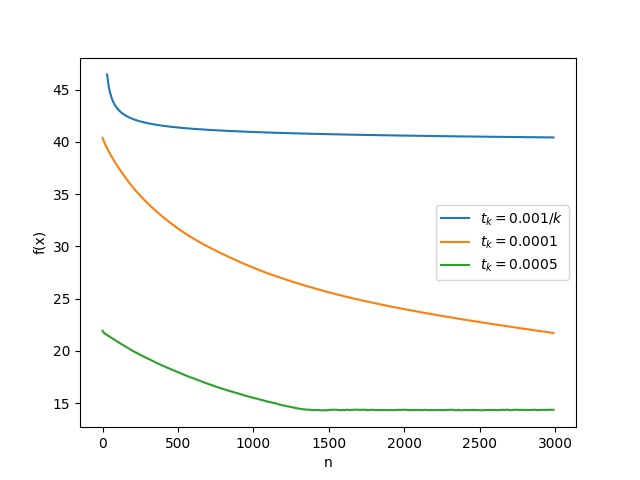
\includegraphics[width=1\textwidth]{subgradient3000.jpg}
\caption{Iteration 3000}
\end{minipage}
\hfill
\begin{minipage}[t]{0.3\linewidth}
\centering
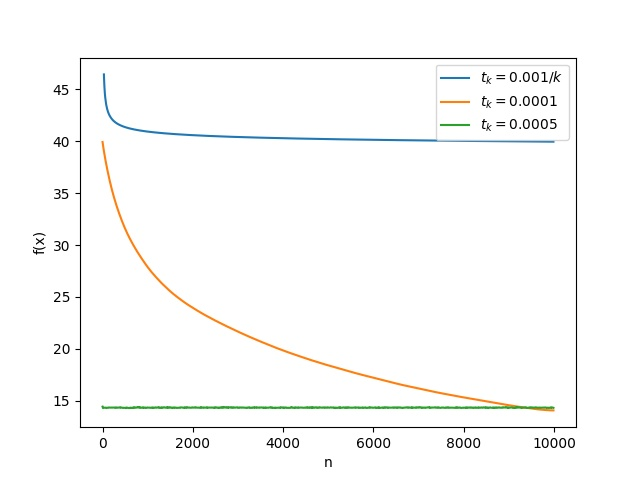
\includegraphics[width=1\textwidth]{subgradient10000.jpg}
\caption{Iteration 10000}
\end{minipage}
\begin{minipage}[t]{0.3\linewidth}
\centering
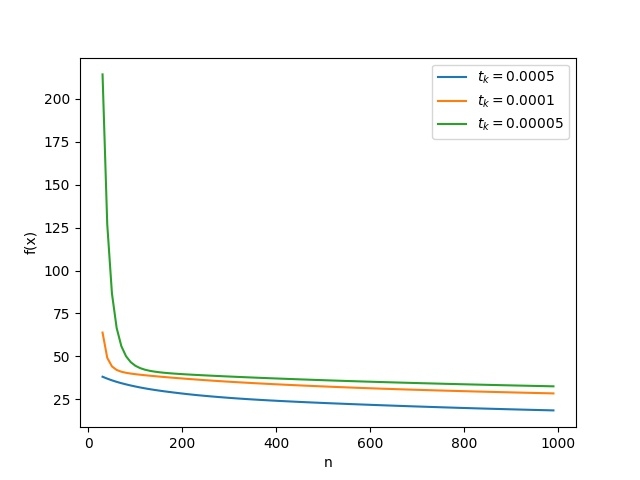
\includegraphics[width=1\textwidth]{subgradient100000.jpg}
\caption{Iteration 100000}
\end{minipage}
\end{figure}
\begin{footnotesize}
\begin{minted}{python}

import numpy as np
import matplotlib.pyplot as plt

def partial(x):
    res=np.zeros((len(x),1))
    for i in range(len(x)):

        if abs(x[i])<eps:
                res[i]=0
        else:
            res[i]=x[i]/abs(x[i])

    tmp=A.dot(x)-b
    res2=A.T.dot(tmp)
    return res+res2

def f(x):
    s1=0
    for i in range(len(x)):
        s1+=abs(x[i])
    tmp=A.dot(x)-b
    s2=np.dot(tmp.T,tmp)
    return s1+s2


np.random.seed(1000)
eps=1e-7
m=200
n=1000
A=np.random.normal(0,1,(m,n))
x_bar=np.zeros((n,1))
for i in range(20):
    k=np.random.randint(0,1000)
    x_bar[k]=np.random.normal(0,1)
b=A.dot(x_bar)

x_pre=np.zeros((n,1))
x_now=x_pre
y1=[]
n1=[]
y2=[]
n2=[]
y3=[]
n3=[]
iteration=100000
for i in range(iteration):
    tk=0.001/(i+1)
    x_now=x_pre-tk*partial(x_pre)
    x_pre=x_now
    if i%10==0 and i>20:
        y1.append(f(x_now)[0][0])
        n1.append(i)
for i in range(iteration):
    tk=0.0001
    x_now=x_pre-tk*partial(x_pre)
    x_pre=x_now
    if i%10==0:
        y2.append(f(x_now)[0][0])
        n2.append(i)
for i in range(iteration):
    tk=0.0005
    x_now=x_pre-tk*partial(x_pre)
    x_pre=x_now
    if i%10==0:
        y3.append(f(x_now)[0][0])
        n3.append(i)
plt.plot(n1,y1,label=r'$t_{k}=0.001/k$')
plt.plot(n2,y2,label=r'$t_{k}=0.0001$')
plt.plot(n3,y3,label=r'$t_{k}=0.0005$')
plt.xlabel("n")
plt.ylabel("f(x)")
plt.legend()
plt.savefig("subgradient100000.jpg")
plt.show()

\end{minted}
\end{footnotesize}
\subsection*{2.}
Let $\bm{a}=\bm{x}^{k-1}-\bm{x}^{k-2}$,$\bm{b}=\nabla f(\bm{x}^{k-1})-\nabla f(\bm{x}^{k-2})$
$$f(\frac{1}{t})=||{\bm{a}}/{t}-\bm{b}||_{2}^{2}$$
Let $$\frac{\partial f}{\partial 1/t}=0$$
we get $\hat{t}=\bm{a}^{\mathrm{T}}\bm{a}/\bm{a}^{\mathrm{T}}\bm{b}$.

In the same way, we get $\tilde{t}=\bm{a}^{\mathrm{T}}\bm{b}/\bm{b}^{\mathrm{T}}\bm{b}$

Because $\nabla f(\bm{x})$ is Lipschitz continuous with $L$, $\frac{L}{2}\bm{x}^{\mathrm{T}}\bm{x}-f(\bm{x})$ is convex. $L\bm{x}-\nabla f(\bm{x})$ is monotone, which is equivalent to $\hat{t}\geq 1/L$.Because of the co-coercivity, we get $\tilde{t}\geq 1/L$. So $\mathrm{min}\{\hat{t},\tilde{t}\} \geq 1/L$

\subsection*{3.}


Suppose $\bm{y}=\mathrm{prox}_{f}(\bm{x}),\bm{x}=(x_{1},x_{2},\cdots ,x_{n})^{\mathrm{T}},\bm{y}=(y_{1},y_{2},\cdots , y_{n})^{\mathrm{T}}$.
\subsubsection*{1}

$$y_{i}=\left\{
\begin{aligned}
&1& \mathrm{if}&\ \ \  x_{i}> 2\\
&x_{i}-1 & \mathrm{if}&\ \ \  1\leq x_{i}\leq2\\
&0& \mathrm{if}&\ \ \  -1<x_{i}<1\\
&x_{i}+1 & \mathrm{if}&\ \ \  -2 \leq x_{i}\leq-1\\
&-1 & \mathrm{if}&\ \ \  x_{i}<-2
\end{aligned}
\right.
$$
\subsubsection*{2}
Consider $g(\bm{x})=||\bm{x}||_{1}$. $f(\bm{x})=g(A\bm{x}-\bm{b})$. Suppose $AA^{\mathrm{T}}=\mathrm{diag}(\lambda_{1},\lambda_{2},\cdots,\lambda_{n})$, where $C=\mathrm{diag}(\sqrt{\lambda_{1}},\sqrt{\lambda_{2}},\cdots,\sqrt{\lambda_{n}})$. We have $C^{2}=AA^{\mathrm{T}}$.

$\bm{u}=\mathrm{prox}_{f}(\bm{x})$ is the solution of the optimization problem
$$\min_{\bm{u},\bm{v}}g(\bm{v})+\frac{1}{2}||\bm{u}-\bm{x}||_{2}^{2} \ \ \ \ \mathrm{s.t.}\ \ A\bm{u}-\bm{b}=\bm{v}$$
Lagrangian function: $$L(\bm{u},\bm{v},\bm{\lambda})= g(\bm{v})+\frac{1}{2}||\bm{u}-\bm{x}||_{2}^{2}+\bm{\lambda}^{\mathrm{T}}(A\bm{u}-\bm{b}-\bm{v})$$
KKT conditions:
$$\bm{u}-\bm{x}+A^{\mathrm{T}}\bm{\lambda}=\bm{0}$$
$$\bm{\lambda}\in \partial g(\bm{v})$$
$$A\bm{u}-\bm{b}=\bm{v}$$
So $$\bm{0}\in \partial g(\bm{v})+(AA^{\mathrm{T}})^{-1}(\bm{v}-(A\bm{x}-\bm{b}))$$,
which means $\bm{v}$ is the minimizer of $h(\bm{v})=g(\bm{v})+1/2||C^{-1}\bm{v}-C^{-1}(A\bm{x}-b)||^{2}_{2}$.
Because $C$ is diagonal matrix, $g(\bm{v})=||\bm{v}||_{1}$. It is separable for $$h(\bm{v})=\sum_{i=1}^{n}|v_{i}|+\frac{1}{2}(\frac{v_{i}}{\sqrt{\lambda_{i}}}-C^{-1}(A\bm{x}-b)[i])$$
So we can get the minimizer $\hat{\bm{v}}$.
\begin{align*}
\mathrm{prox}_{f}(\bm{x})&=\bm{u}\\
&=\bm{x}-A^{\mathrm{T}}\bm{\lambda}\\
&=\bm{x}-A^{\mathrm{T}}(AA^{\mathrm{T}})^{-1}(A\bm{x}-\hat{\bm{v}}-\bm{b})
\end{align*}
\subsubsection*{3}
For any $\bm{x}=(x_{1},x_{2},\cdots,x_{n})^{\mathrm{T}}$.Note that $x_{k_{i}}$ is the $i$-th largest component in the vector $\bm{x}$, $k_{i}$ is the index of the $i$-th largest component in the vector $\bm{x}$. For example, if $\bm{x}=(2,4,1,5)^{\mathrm{T}}$, then $x_{k_{1}}=5, k_{1}=4$.

$\bm{y}=\mathrm{prox}_{f}(\bm{x})$. We have $y_{k_{1}}=x_{k_{1}}-1$, $y_{k_{i}}=x_{k_{i}},i>1$.

\subsubsection*{4}
$$\bm{y}=\left\{
\begin{aligned}
&(1-1/||\bm{x}||)\bm{x}&\mathrm{if}\ \ \ &||\bm{x}||<1\\
&\bm{0}&\mathrm{if}\ \ \ &1\leq||\bm{x}||\leq3\\
&(1+1/||\bm{x}||)\bm{x}&\mathrm{if}\ \ \ &||\bm{x}||>3
\end{aligned}
\right.
$$
\subsubsection*{5}

Suppose $X$ has SVD $X=P\mathrm{diag}(\lambda_{1},\cdots,\lambda_{n})Q^{\mathrm{T}}$,
$\bm{\lambda}=(\lambda_{1},\cdots,\lambda_{n})^{\mathrm{T}}$.

Let $$\hat{\bm{\lambda}}=\mathop{\arg\min}_{\bm{u}}||\bm{u}||_{1}+\frac{1}{2}||\bm{u}-\lambda||_{2}^{2}$$
The proximal mapping is $$\mathrm{prox}_{f}(X)=P\mathrm{diag}(\hat{\lambda_{1}},\cdots,\hat{\lambda_{n}})Q^{\mathrm{T}}$$
\subsection*{4.}
Let $$g(\bm{x})=\sup_{\bm{u}}(-f(\bm{u})-\frac{1}{2\lambda}||\bm{u}||_{2}^{2}+\frac{1}{\lambda}\bm{u}^{\mathrm{T}}\bm{x})$$
$\bm{u}^{*}$ is the maximizer, $\bm{0}\in \partial\lambda f(\bm{u}^{*})+\bm{u}^{*}-\bm{x}$, so
$$\bm{u}^{*}=\mathop{\arg\min}_{\bm{u}}\lambda f(\bm{u})+\frac{1}{2}||\bm{u}-\bm{x}||_{2}^{2}=\mathrm{prox}_{\lambda f}(\bm{x})$$

Thus,
\begin{align*}
\nabla f_{\lambda}(\bm{x})&=\frac{\bm{x}}{\lambda}-\nabla g(\bm{x})\\
&=\frac{\bm{x}}{\lambda}-\mathrm{prox}_{\lambda f}(\bm{x})
\end{align*}
\end{document}
